\part{Backend}
\label{backend}

\chapter{Allgemeines}

Der \textbf{Backend-Server} hat die Aufgabe, durch fest definierte Zugangspunkte den Abruf oder die Veränderung von Daten in der Datenbank des Systems zu ermöglichen. Damit das funktioniert besteht der Server aus zwei ganz grundlegenden Teilen:

\begin{itemize}
    \item \textbf{Datenbankverbindung}
    \item \textbf{REST-API}
\end{itemize}

Für die Implementation des Servers wurde die von Microsoft entwickelte Scriptsprache \textit{\nameref{typescript}} gewählt. Der Code davon wird anschließend mit Hilfe von \textit{\nameref{gulpjs}} zu \textit{\nameref{javascript}} kompiliert.

\section{Datenbankverbindung}

Zum Start der Anwendung versucht der Server mit Hilfe der Library \lstinline{mysql} eine Verbindung zum MySQL-Server aufgebaut, welcher in einem anderen Docker-Container läuft. MySQL nutzt als Hostname den Containernamen, weshalb der Server via \lstinline{mysql:3306} eine Verbindung zu MySQL herstellen kann. Die Anmeldedaten für MySQL werden sicher in \textit{\nameref{dockersecrets}} gespeichert.

\section{Konfiguration}

Der Backend-Server erlaubt einige Konfigurationsmöglichkeiten. Werte für Konfigurationen werden zuerst aus den Umgebungsvariablen geladen. Sofern dort kein Wert gefunden werden kann, wird der Wert in \textit{\nameref{dockersecrets}} gesucht.

\subsection{Verfügbare Konfigurationen}

\lstinline{DEBUG: boolean} \\
$\rightarrow$ aktiviert den Debug-Modus. Dieser muss für lokale Tests immer \lstinline{true} sein! Ist dieser Wert \lstinline{true}, so werden beispielsweise Bilder in einem lokalen \lstinline{images}-Ordner gespeichert und nicht in der Docker Volume.

\lstinline{DEBUG_LOG: boolean} \\
$\rightarrow$ aktiviert den Debug-Log. Ist dieser Wert auf \lstinline{true} werden beispielsweise alle eingehende Anfragen an den Server im Log mitgeschrieben.

\lstinline{DOMAIN: string} \\
$\rightarrow$ ist die Domain, unter dem der Backend-Server erreichbar ist. Wird genutzt, um in Verifikations-E-Mails die richtige Domain zu senden.

\lstinline{MAX_USER_SESSIONS: number} \\
$\rightarrow$ gibt an, wie oft sich ein Nutzer (z. B. bei einem neuen Gerät) anmelden kann, bevor eine Session ungültig gemacht wird.

\lstinline{MAX_ACP_USER_SESSIONS: number} \\
$\rightarrow$ gibt an, wie oft sich ein ACP-Nutzer (z. B. bei einem neuen Gerät) anmelden kann, bevor eine Session ungültig gemacht wird.

\lstinline{SALT_ROUNDS: number} \\
$\rightarrow$ gibt an, wie oft \lstinline{bcrypt} ein Passwort oder einen Session-Token hasht, bevor er in die Datenbank gespeichert wird. Je größer dieser Wert ist, desto schwieriger ist es, den Hash zu "erraten". \lstinline{10} ist hierfür meist ein sicherer Wert. \cite{stoeckli2017}

\subsection{Docker Secrets}
\label{dockersecrets}

\textbf{Docker Secrets} erlaubt es, sensitive Daten wie Passwörter oder Zugangsschlüssel sicher auf einem Server zu speichern. Im Fall von Sokka werden \lstinline{MYSQL_DB}, \lstinline{MYSQL_HOST}, \lstinline{MYSQL_USERNAME}, \lstinline{MYSQL_PASSWORD}, \lstinline{VERIFY_EMAIL} und \lstinline{VERIFY_EMAIL_PASSWORD}. 

Die Secrets müssen in Textdateien in einem vom VCS ausgenommenen Ordner erstellt werden. Diese Textdateien müssen anschließend bei der Erstellung der Container, in unserem Fall in der \lstinline{docker-compose.yml}, eingetragen werden. Beim Start der Container werden alle Secrets in die Container an den Pfad \lstinline{/run/secrets/<key>} kopiert, wo sie schlussendlich ausgelesen werden können.

\begin{code}[htp]
    \begin{center}
        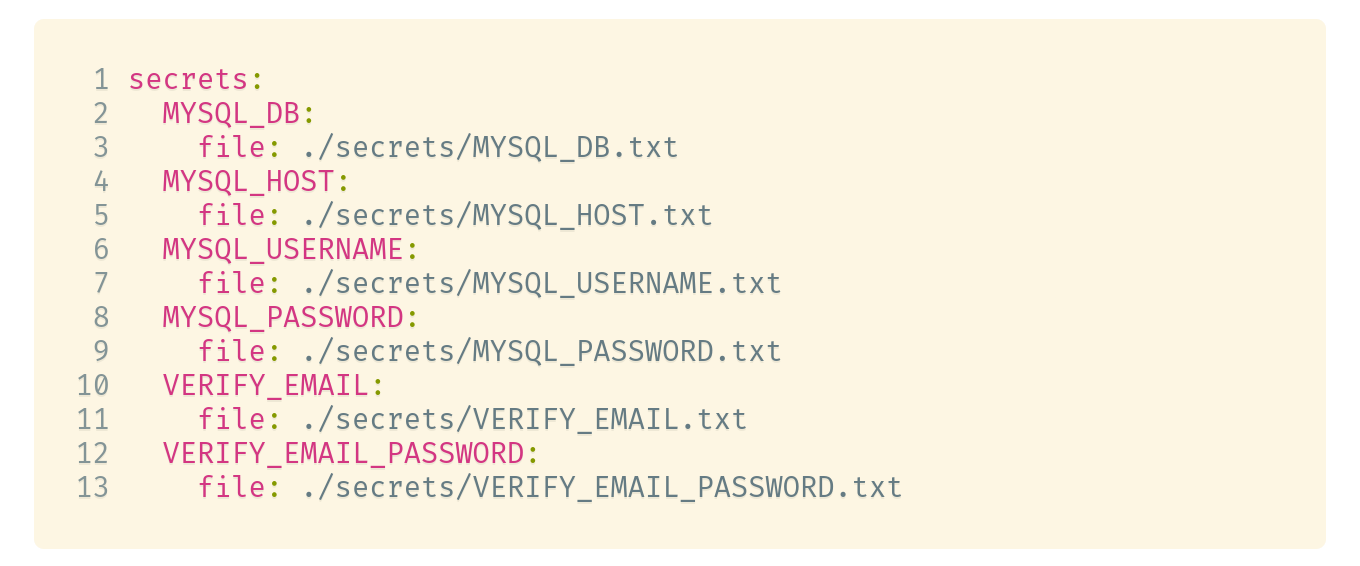
\includegraphics[width=1\textwidth]{images/Backend/secrets.png}
        \vspace{-25pt}
        \caption{Sokkas Docker Secrets in der \lstinline{docker-compose.yml}}
    \end{center}
\end{code}

\section{REST-API}

Damit die \textit{\nameref{client}} und das \textit{\nameref{acp}} auch auf die Daten der Datenbank zugreifen können stellt der Server dokumentierte Zugangspunkte oder auch \textbf{REST-Routes} zur Verfügung. Computer im Internet können auf diese Routes zugreifen, indem sie vorgefertige HTTP-Anfragen an den Server senden. Wie genau diese Anfragen aussehen müssen, wird im Kapitel \textit{\nameref{restdoc}} genauer erläutert.

\subsection{Bilder}

Sowohl Produkte als auch Menüs erhalten in Sokka anpassbare Bilder. Um dies zu realisieren existiert \textit{\nameref{acpimage}} zum Hochladen von Bildern und \textit{\nameref{image}} zum Abrufen von Bildern.

Wenn ein Bild über die ACP-Route hochgeladen wird, legt der Server das Bild mit einer zufallsgenerierten ID (16 Bytes, Hex enkodiert) in einer Docker Volume ab. Diese Bilder können dann später wieder über die zweite Route abgerufen werden.

\subsection{Verifikation}

Bei der Registrierung müssen Nutzer ihre E-Mail-Adresse angeben. Um sicherzugehen, dass diese Adresse auch wirklich gültig ist, wurde mit Hilfe der Library \textit{nodemailer} ein simples E-Mail-Verifikationssystem implementiert. Ein Nutzer kann erst Bestellungen tätigen, wenn sein Nutzerkonto verifiziert ist.

Schon beim Start des Servers wird geprüft, ob die in den \textit{\nameref{dockersecrets}} gespeicherten Informationen zur Anmeldung bei Google-Mail korrekt sind (\lstinline{VERIFY_EMAIL} und \lstinline{VERIFY_EMAIL_PASSWORD}). \lstinline{VERIFY_EMAIL_PASSWORD} ist hier allerdings nicht wirklich das Passwort für das Google-Mail-Konto, sondern ein generiertes App-Passwort (myaccount.google.com/u/1/apppasswords).

Sofern die gespeicherten Anmeldedaten korrekt sind (und der Anmeldevorgang bei Google erfolgreich war), kann der Server vollautomatisch E-Mails an neue Nutzer versenden.

Wenn sich ein neuer Nutzer durch die REST-Route \textit{\nameref{usercreate}} mit einer laut RFC 5322 gültigen E-Mail-Adresse registriert, werden 64 zufällige Bytes generiert, welche anschließend in Base64 enkodiert werden und der entstandene String in Verbindung mit der ID des Nutzerkontos in einer Tabelle abgelegt.

Im selben Moment wird an die angegebene E-Mail-Adresse eine Nachricht mit einer URL gesendet, welche den generierten String enthält.

\begin{figure}[htp]
    \begin{center}
        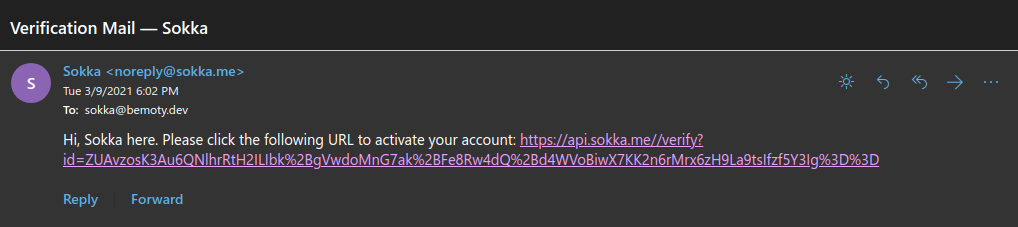
\includegraphics[width=1\textwidth]{images/Backend/mail.png}
        \caption{Eine E-Mail, welche durch Sokka bei der Verifizierung gesendet wurde}
    \end{center}
\end{figure}

Die URL in der E-Mail führt zur REST-Route \textit{\nameref{verify}}, welche, wenn der String in der URL gültig ist, das damit verbundene Nutzerkonto verifiziert.

\section{ACP-User-Authentication}

Grundsätzlich ist die Authentifikation eines Nutzers zur Verwendung des Admin-Clients
gleich aufgebaut, wie jene des normalen Clients.

Die Anmeldedaten werden über Textfelder vom Nutzer eingegeben und per Druck des Submit-Buttons
zur Überprüfung an den Server gesendet.\\
Ist der Anmeldevorgang erfolgreich, wird ein Session-Token übermittelt, der als Cookie
im Gerät abgespeichert wird.